% !TeX spellcheck = en_GB

\pgfplotsset{compat=1.17}

\begin{frame}{About Me}
	\begin{columns}
		
		\begin{column}{0.45\textwidth}
			\begin{tcolorbox}[colback=white, colframe=ElixirPurple, arc=3mm, boxrule=0mm, height=0.8\textheight, valign=center, title=Working Live]
				
				\underline{topics}:
				\begin{itemize}
					\item heat demand and PV cadastres
				\end{itemize}
				\underline{using}:
				\begin{itemize}
					\item geodata (Raster, Vector)
					\item Python: GeoPandas, Numpy
					\item land usage; coverage, property register
				\end{itemize}
				
			\end{tcolorbox}
		\end{column}
		
		\begin{column}{0.45\textwidth}
			\begin{tcolorbox}[colback=white, colframe=ElixirPurple, arc=3mm, boxrule=0mm, height=0.8\textheight, valign=center, title=Privat Live]
				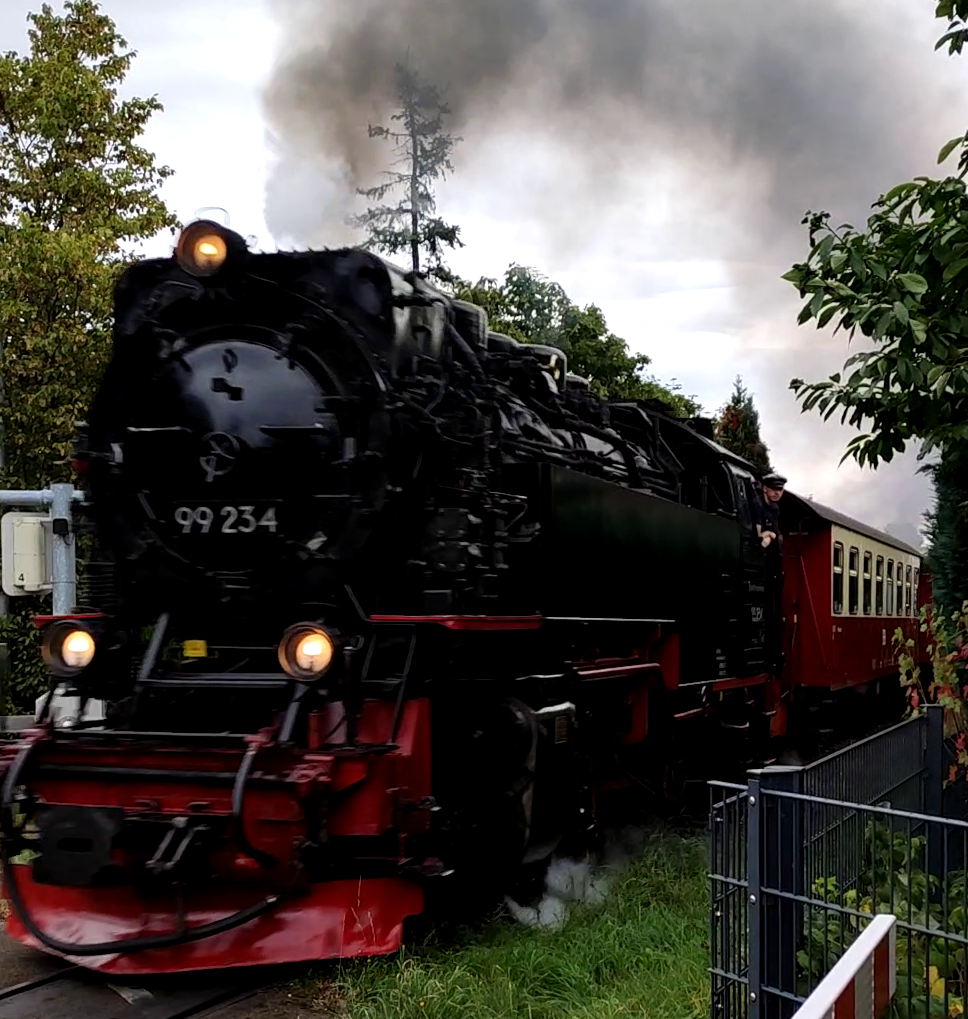
\includegraphics[width=\tcbtextwidth,   keepaspectratio]{pictures/vlcsnap-2024-01-31-23h37m06s479.png}
			\end{tcolorbox}
		\end{column}
		
	\end{columns}
\end{frame}